\section{Alex Pitcher Report - Kate Smith}

\margininbox{Alex Pitcher, 2010}{Kate Smith's report for the Alex Pitcher memorial fund award.}{\award}


From 15\(^{th}\) July to 15\(^{th}\) August 2010, I joined Imperial College Caving Club on their summer expedition
to the Julian Alps to explore the expansive Slovenian cave systems there. ICCC have been present
in the area almost annually since 1994, running joint exploration with a local club from the town
of \passage[town]{Tolmin}, the JSPDT. From \passage[town]{Tolmin} we travelled 6km to the large limestone plateau of \passage[mountain]{Tolminski
Migovec}, within the \passage{Triglav national park}. Here I lived for 27 days with various members of the
expedition, united by the sole motive to find and survey virgin cave.



    \begin{marginfigure}
\checkoddpage \ifoddpage \forcerectofloat \else \forceversofloat \fi
\centering
 \frame{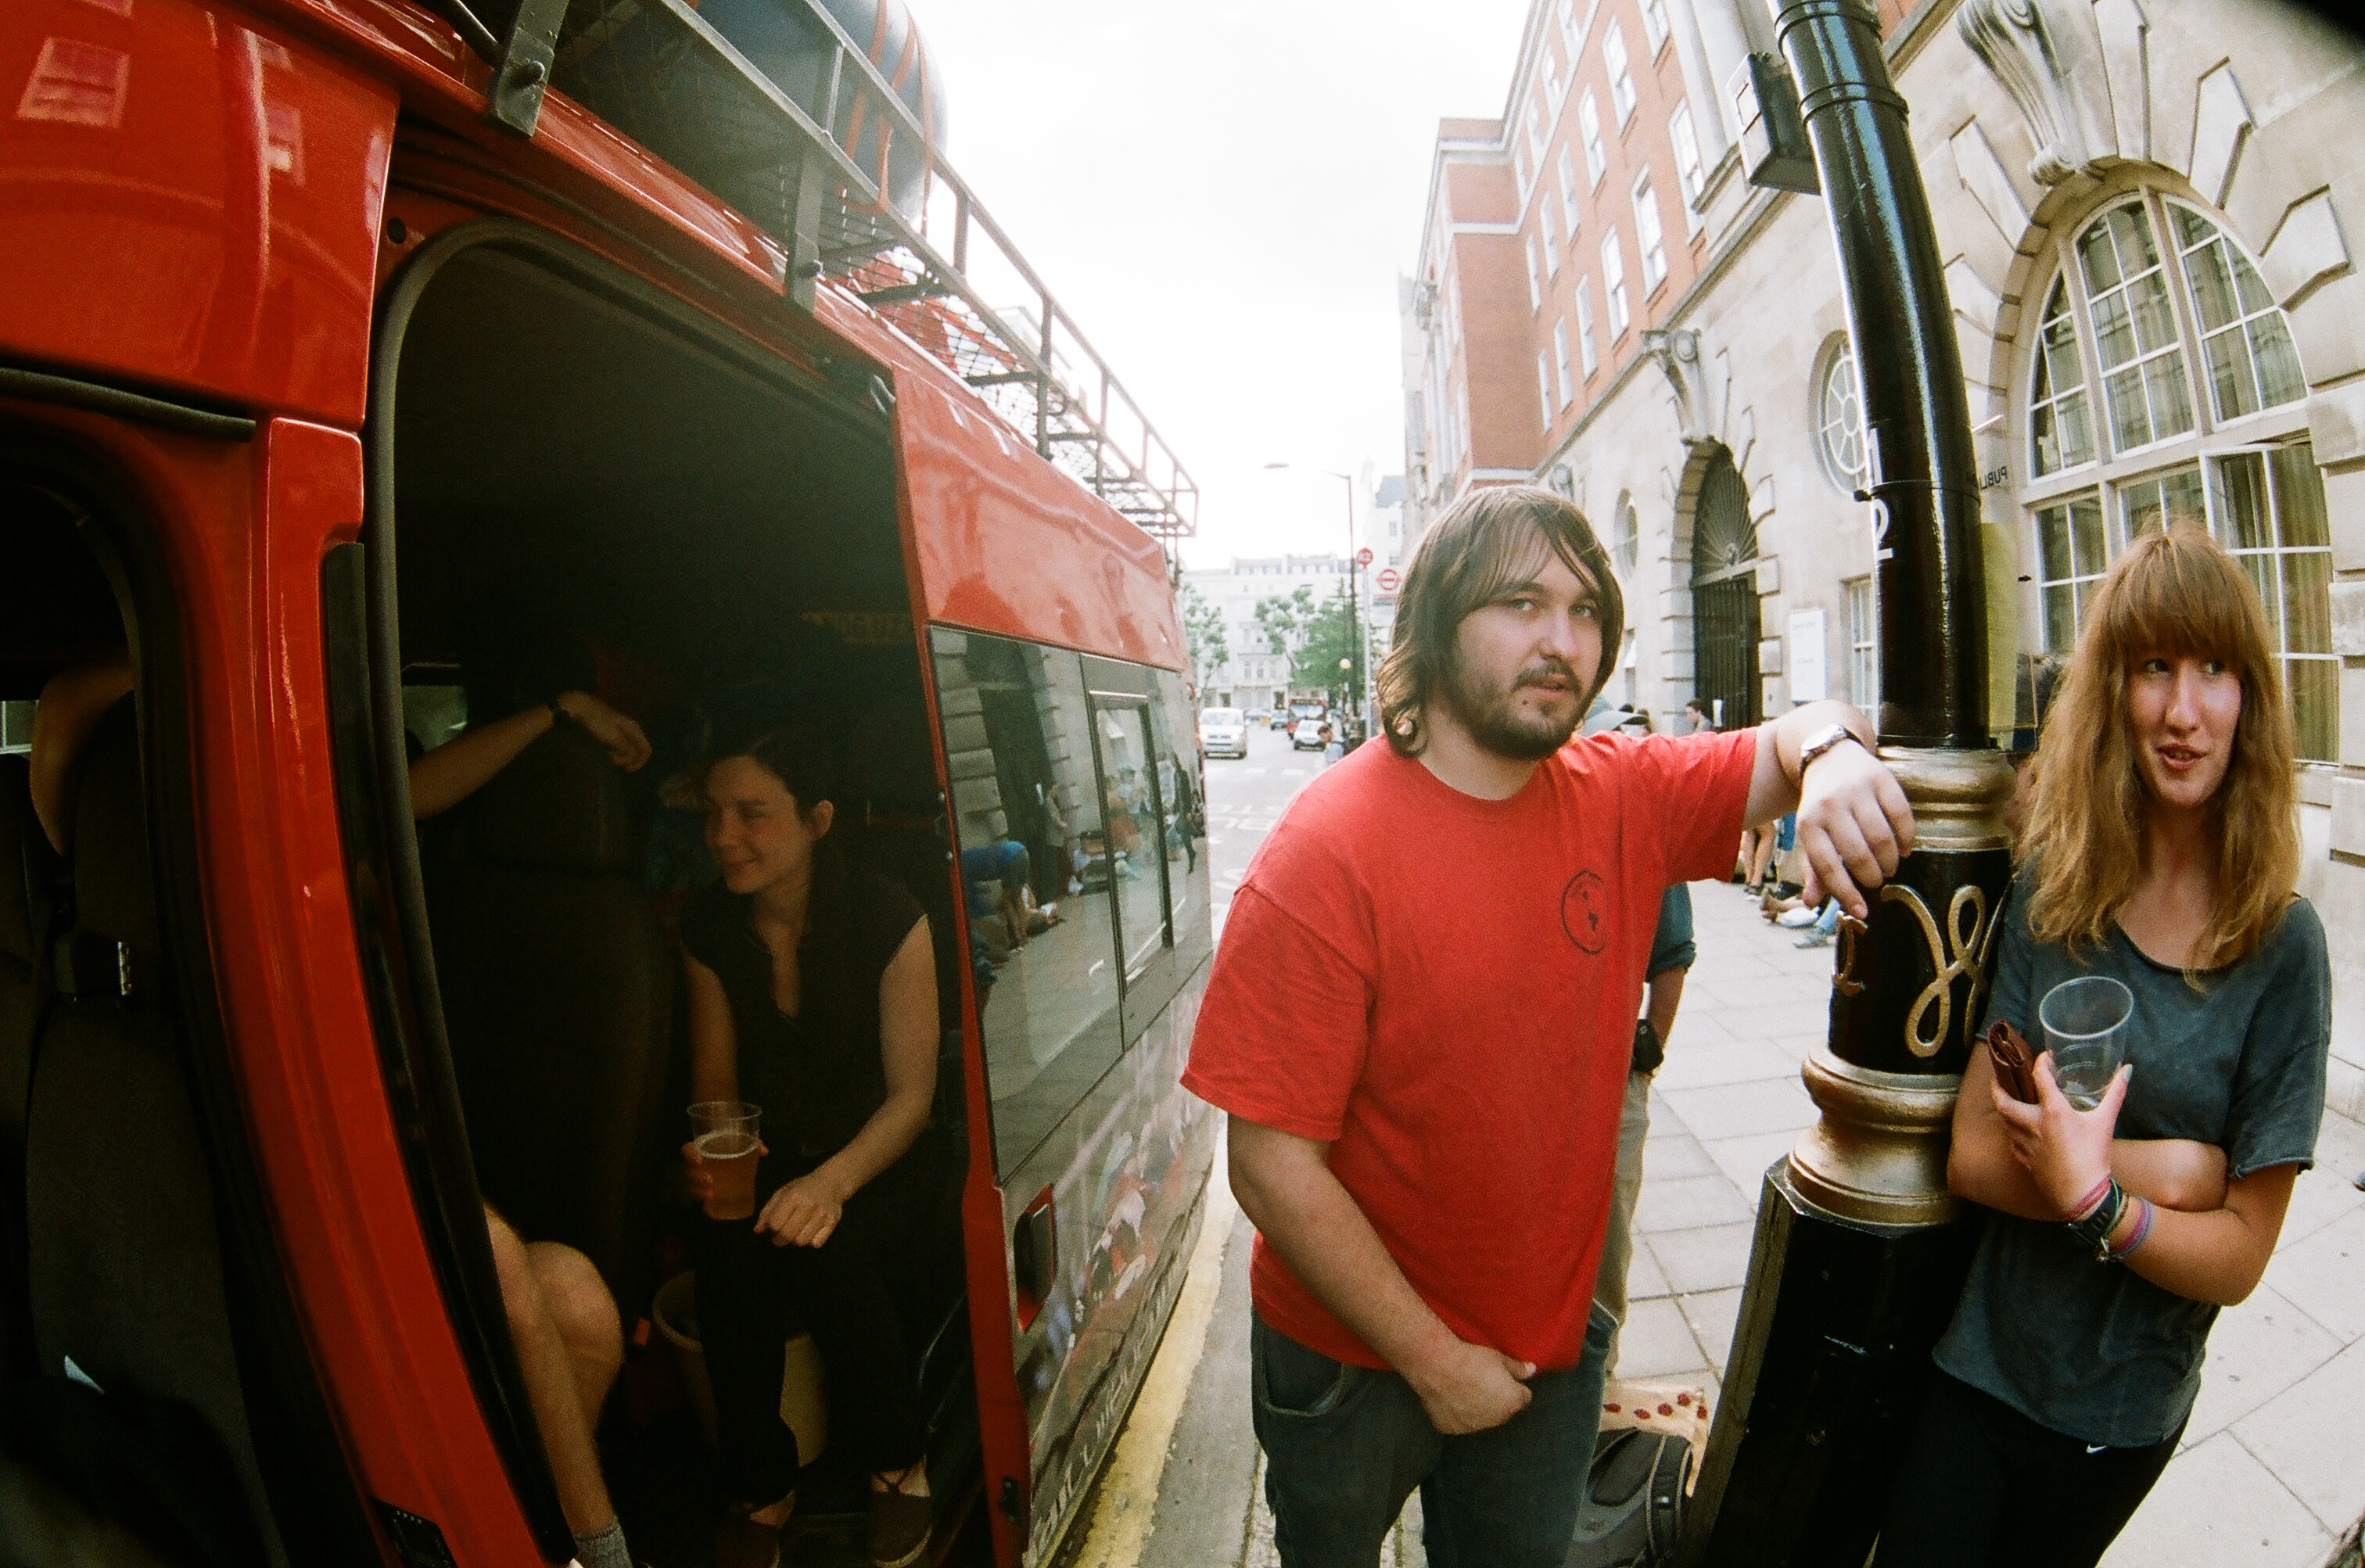
\includegraphics[width=\linewidth]{2010/ap_awards/Jarvist Frost - Canon A1 Zenit 16mm - 61320007--orig.jpg}} 
 \caption{Jana, Alex and Kate outside Imperial College Union before the minibus leaves for Slovenia. \pic{Jarvist Frost}}
 \label{bus union 2010}
\end{marginfigure}


Six of us set off to Slovenia in a university minibus that was jam-packed with 2km of rope, food
and caving equipment. 24 hours after leaving London and passing through France, Belgium, Germany,
Austria and Italy we arrived at a member's flat in \passage[town]{Tolmin}. We were warmly welcomed by the members
of JSPDT and the ICCC members who had arrived some days before to set up camp on the mountain.
As one of three new cavers to the expedition (having been caving for barely a year), I was met with
much excitement and plans for my first caving trip in the mountains.

\tweet{10:24PM Jul 18th, 2010}{Van safely T'min sat evening.Alpine start delayed by thunder. Carries in rain. 15 up the hill,1st slop and tea.Great to be back in the bivi!}


The next morning we drove some way up the mountain to a farm belonging to a family kind enough
to lend us some barn space to keep our supplies and equipment. From here we carried as much as we
could the rest of the way up \passage[mountain]{Migovec} to 1880 m above sea level, each member making several 'carries'
over the course of the expedition.


Camp on Mig consists of tents dotted around the plateau and a communal living space known as
the \passage{Bivi}. The \passage{Bivi} is a nice big shake hole with a little cave and an impressive stone bridge to provide
some shelter. Here we cook, eat, drink and occasionally take naps. Tarpaulin is strategically hung
around the \passage{Bivi} to catch rainwater for consumption. When not underground the members congregate
here to discuss the exploration and organise future trips. Because the depths at which we cave
are so large, there is an underground camp at -550 m with a capacity of four so that teams can rest
between pushing trips.


    \begin{marginfigure}
\checkoddpage \ifoddpage \forcerectofloat \else \forceversofloat \fi
\centering
 \frame{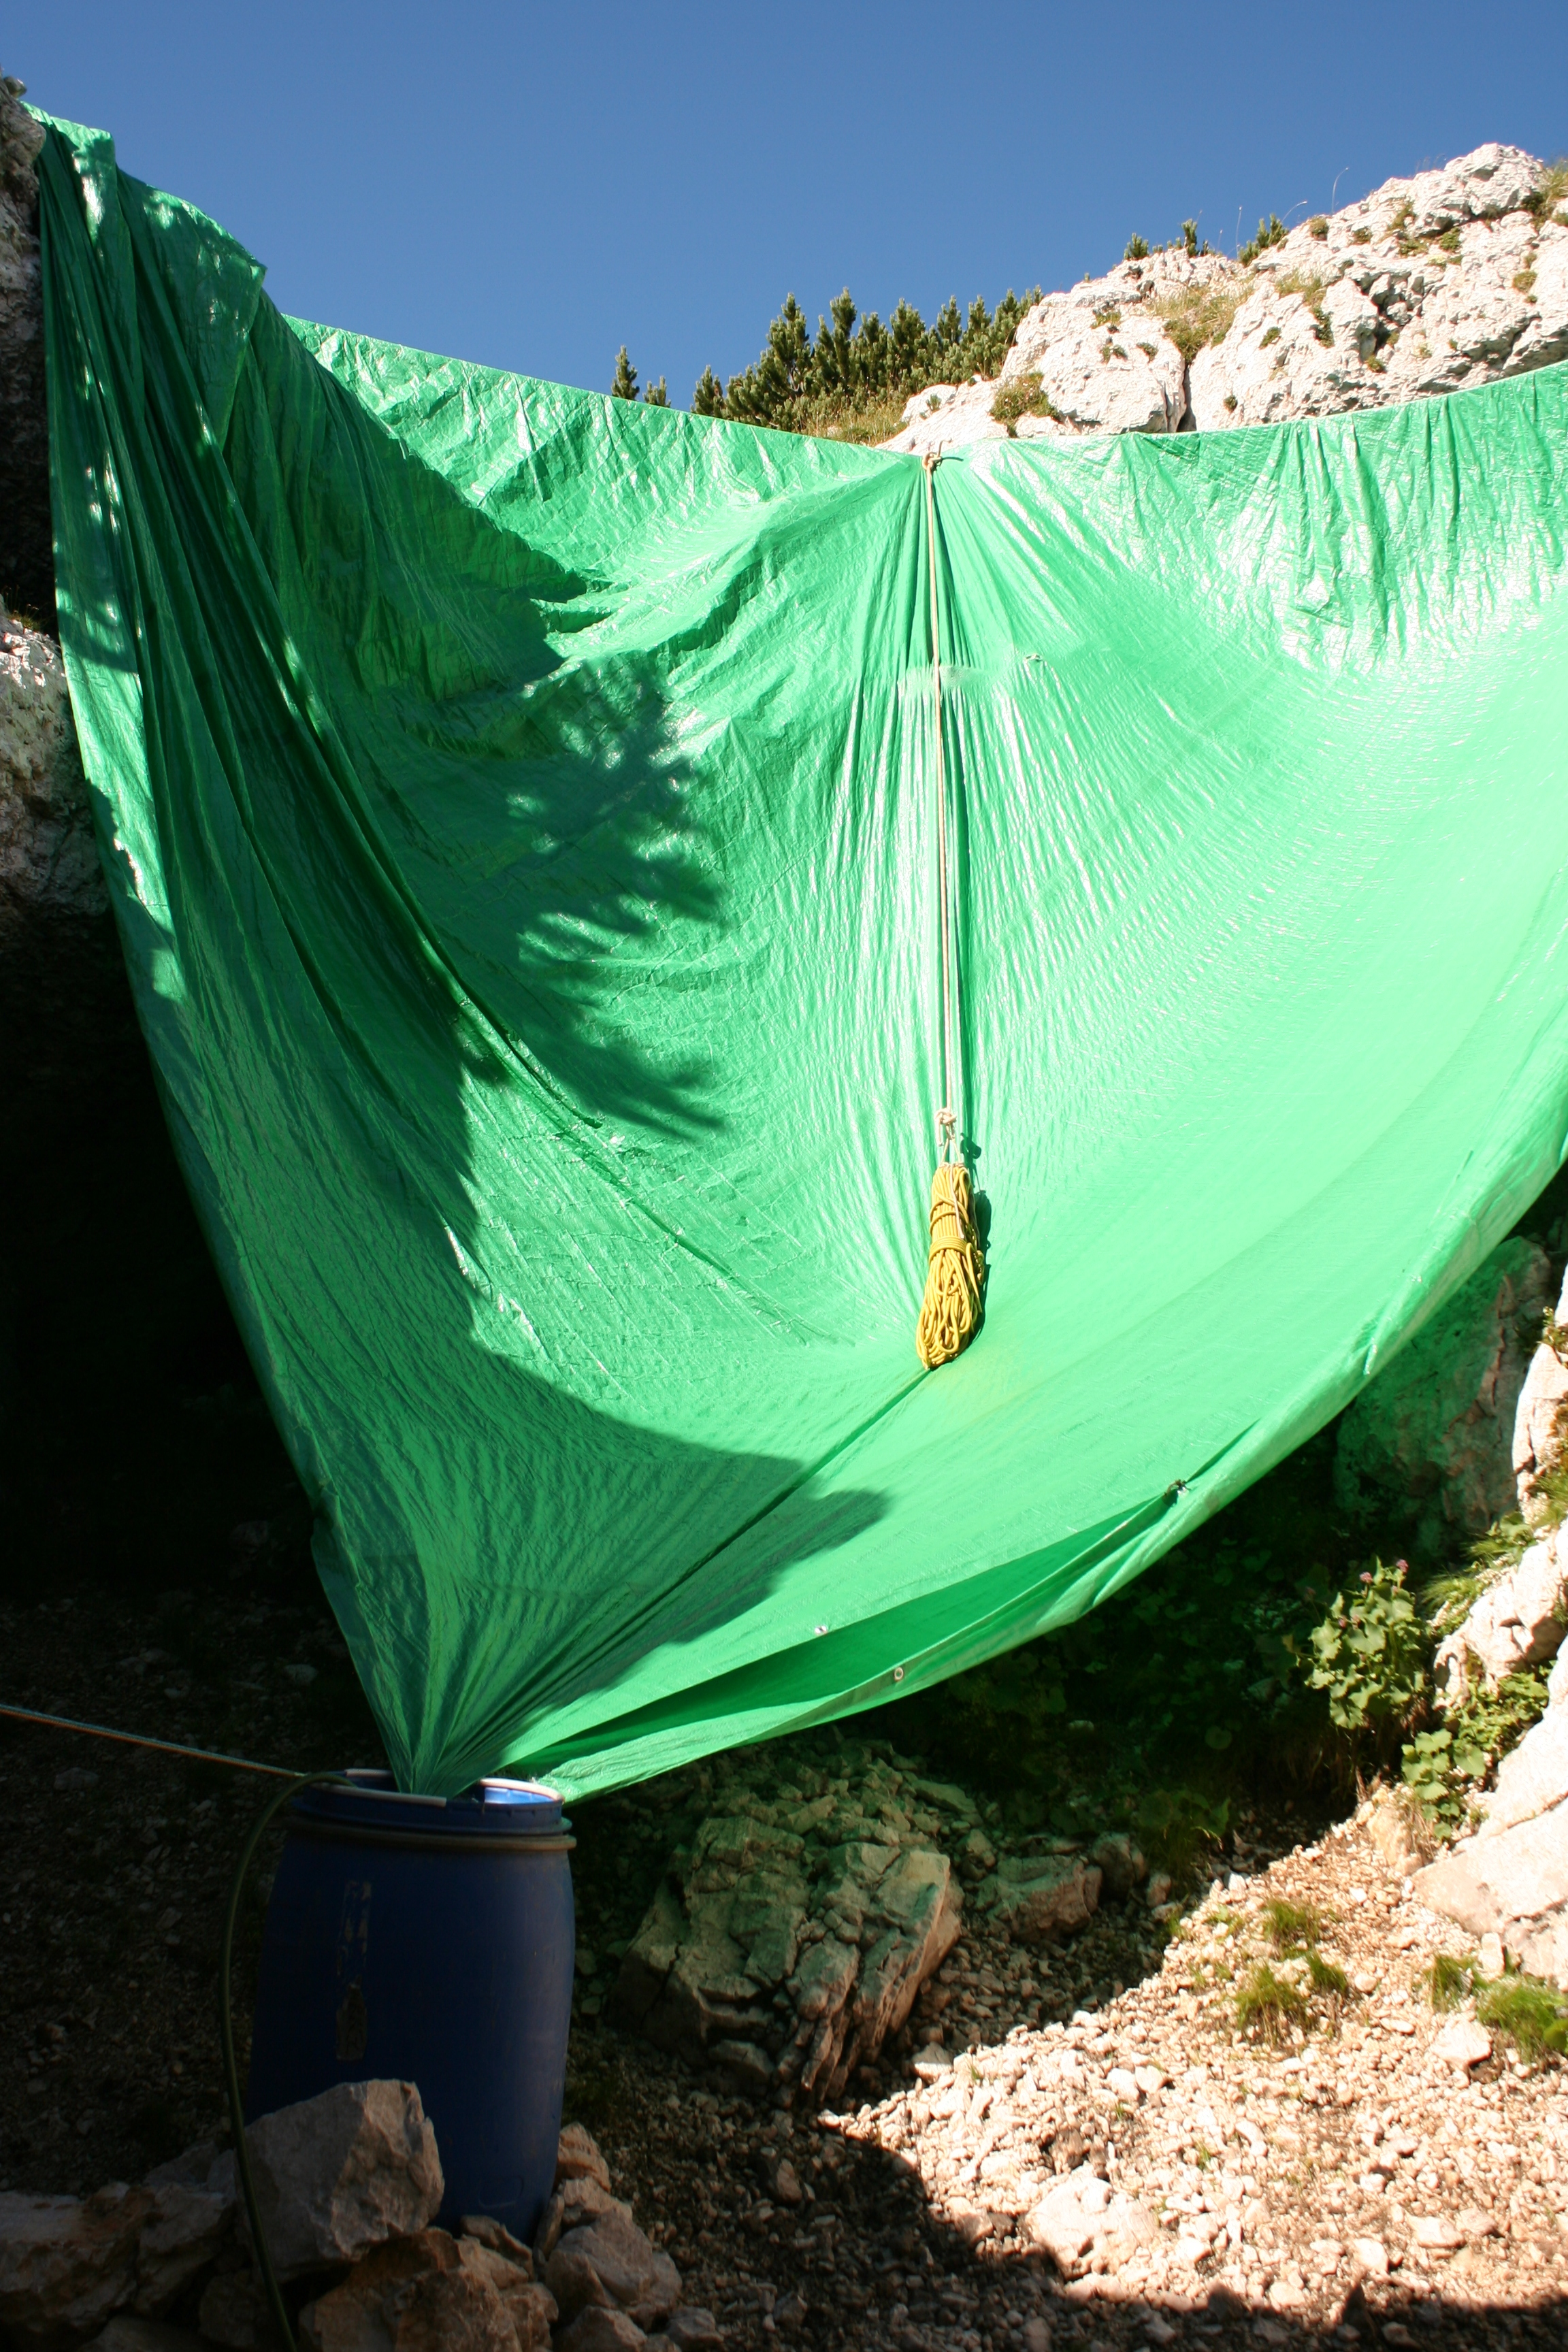
\includegraphics[width=\linewidth]{2010/ap_awards/20100801-07-58-16 - Jana Carga 06--orig.jpg}} 
 \caption{The tarpaulin in the back of the bivi known as the Sail. In 2010 it was brand new and too large, and here is weighed down with a coil of rope to try to prevent its escape across the plateau. \pic{Jana Čarga}}
 \label{sail 2010}
\end{marginfigure}


The initial plan was to introduce us newbies gently to the huge depth of the Slovenian caves with
several trips preparing us for underground camp, although this did not entirely work out. My first
trip was to \passage{Gardener's world}, also known as \passage{Vrtnarija}, one of the two main cave systems in \passage{Migovec}.
Having heard of how Slovene caves differed enormously to British caves I didn't really know what
to expect and found the prospect of entering this alien territory a little daunting. The first thing I
noticed was how sharp and jagged the rocks were so that everything from my oversuit to cowstails got
caught, frustratingly hindering movement. This wasn't too much of a problem though, as the cave is
pleasantly wide and tall with very few passages requiring crawling or squeezing. All of the hard work
is in the large proportion of Single Rope Technique needed. On my first trip we went to -130m, the
depth of a good-sized British cave, and it was lovely and very much in my comfort zone. We had, however, only been down small to medium sized pitches; from where we had turned round, at the top
of a 60m pitch, things further on looked considerably more intimidating.


After a day off from caving due to mad blisters, the opportunity arose to help set up underground
camp. I was initially a bit weirded out by this idea as I came to Slovenia with the eventual goal to make
it to underground camp and now \bignote{I was going to do what I came to do in 3 days time!} However I am
not one to say no to a challenge so hastily made my way underground before I could change my mind.
A team consisting of another eager fresher, two experienced cavers and myself made our way down the
largest pitches I had ever seen, the largest being \passage{Concorde} (my favourite pitch), which at 90m high is
big enough to fit a Concorde in and has the most magnificent limestone formations. After a few hours
and considerably improving my descending technique we made it to the site of underground camp. It
was a long way down and after seeing how much rope we had passed I was dreading prussicking up. I
had never prussicked such a huge distance before, how do I know if I can do it? We quickly set up camp
by pitching the tent, making the beds and unpacking food. We brought a MP3 player and speakers
down so that any fears or panic in my head were soon drowned out by happy music and dancing. One
thing I learnt from my month in Slovenia is that David Bowie can make any dire situation a happy
one. After having some food and listening to the oh-so-homely Blackadder we went to sleep, 550 m
beneath (almost) solid rock and completely disconnected from the world.



    \begin{marginfigure}
\checkoddpage \ifoddpage \forcerectofloat \else \forceversofloat \fi
\centering
 \frame{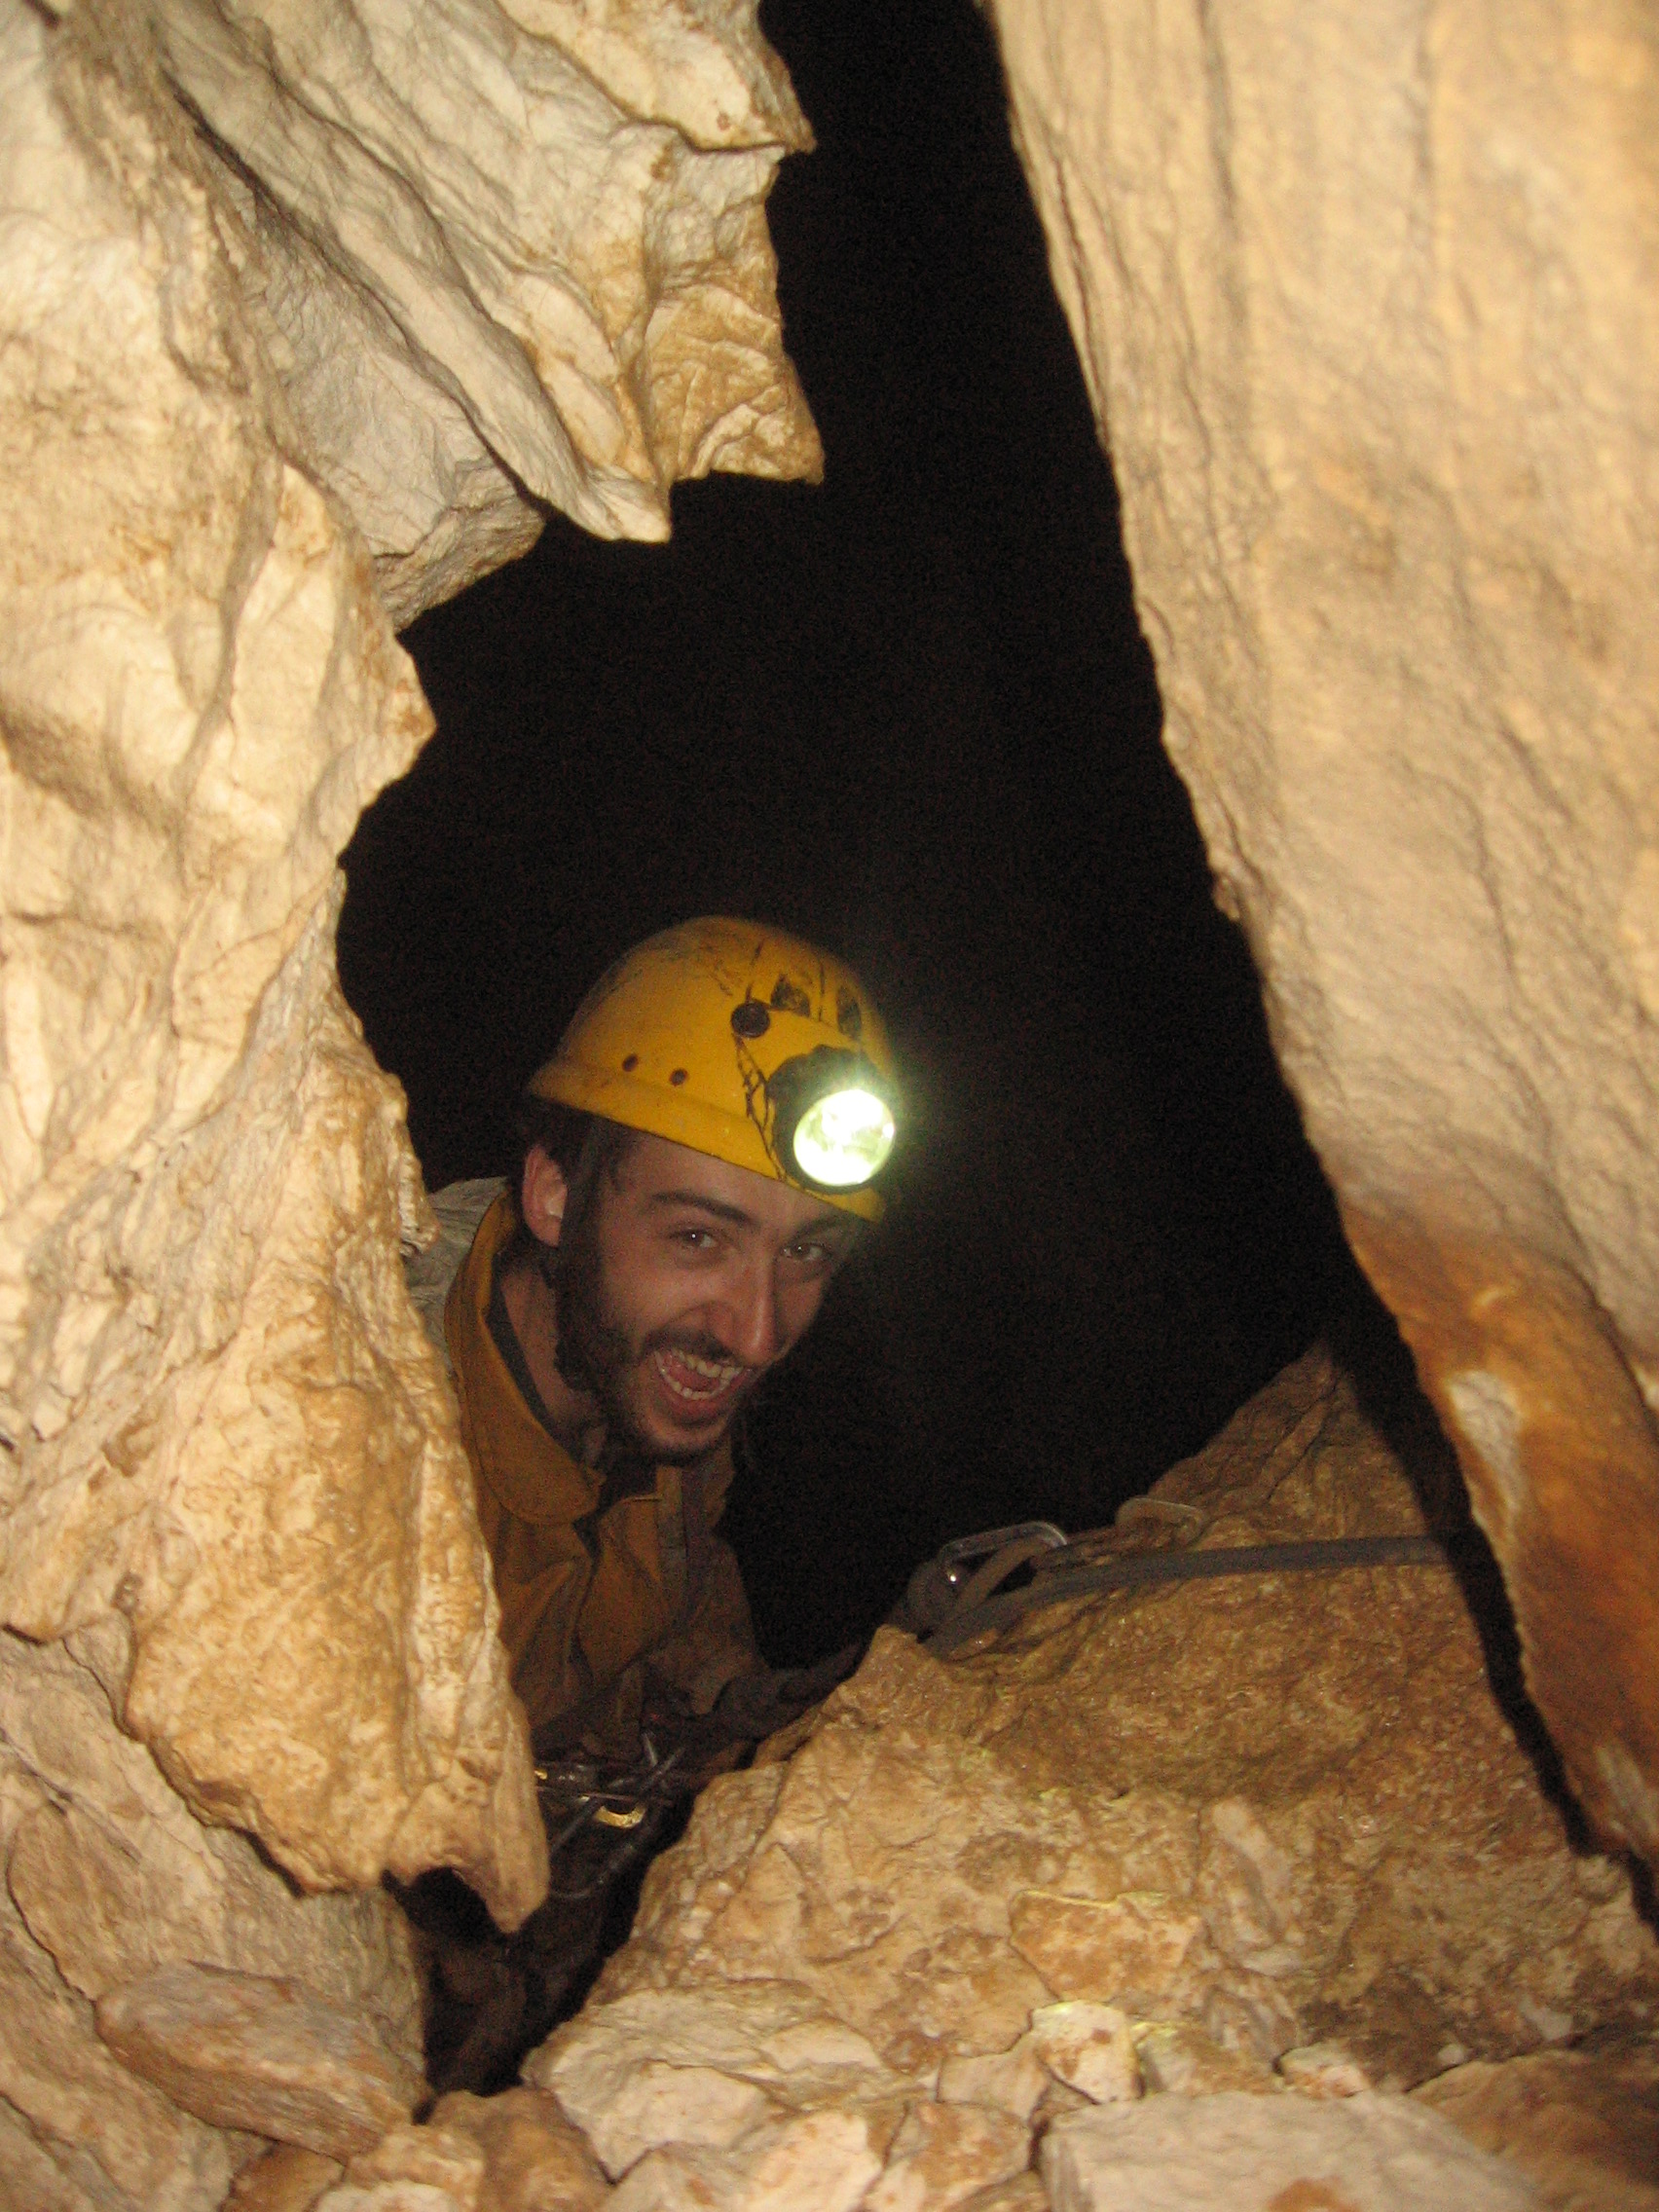
\includegraphics[width=\linewidth]{2010/ap_awards/20100809-15-18-22 - Jarvist Frost A520 - IMG_0008 - Rik on Skynet Rebelay--orig.jpg}} 
 \caption{Rik Venn on \protect\passage{Skynet}. \pic{Jarvist Frost}}
 \label{rik skynet}
\end{marginfigure}


We were awoken by members who were on the night train (caving at night, sleeping in the day) --
they had already been pushing and wanted our beds. We reluctantly crawled out of our snugly sleeping
bags into the 1$^{\circ}$C cold and quickly changed into our cold and wet caving gear. Next was the gruelling
ascent. Due to fear of exhausting myself I adopted a relaxed pace, taking a whopping 8 hours to get
out of the cave. Unfortunately for the member behind, this meant waiting for me and led to attempts
to speed me up such as force feeding me chocolate and even singing. At the first glimpse of sunlight
I thought I was going to cry with happiness. It's strange that after a mere 24 hours without sunlight
you miss it so much and all that physical effort just to see it again makes it all the more magnificent.
Unfortunately after this feeling subsides you realise things were a lot more exciting underground and
that perhaps \bignote{going back down is on top of the list of things to do}.


The next few days were dedicated to treating blisters, nursing sore hands and resting strained
muscles. When I was suitably fit and there was a bed free in underground camp the time arrived
for my first pushing trip. We went down in a team of three and shortly after entering the cave met
another team who had tales of their discovery of '\passage{Wonderland}', a passage with lots of promising leads
and pretty stals. Knowing these leads were ours to follow we eagerly descended to underground camp.
Some interesting incidents on the way down such as my hair getting jammed in the descender and a
scary slip ensured things stayed exciting. I was glad to be back at underground camp, home sweet
home.

\fullwidthbox{26/7 - Second trip to camp}{

Smoked Mackerel fucking delicious. Just came back from \passage{Leopard} and
\passage{Wonderland}. Pretty exciting stuff. Still a bit cranky, probs
hormonal or just reluctant to be down here after just 1 day on surface.
Being the first one at the bottom of newly rigged pitch was immense,
definitely worth any grimness suffered or to be suffered.
\passage{Wonderland} is magical, like a child's playground but with big
holes and sharp jaggedy rocks. After new pitch gorgeous little streamway
- quite small but not uncomfy. \passage{Serpentine}. Stopped at promising
pitch and did some surveying. This caving lark is pretty good. Good
times dancing with Mike and making mud covering on rock with `K' spelt
with stones. Getting out tomorrow, wonder how long it will be this time
till I'm back\ldots{} 
\name{Kate Smith}}

\margininbox{Serpentine}{
     \begin{itemize}
    \item Kate Smith
    \item Mike Foley
    \item Jarvist Frost
    \end{itemize}}{\explo}


\begin{marginfigure}
\checkoddpage \ifoddpage \forcerectofloat \else \forceversofloat \fi
\centering
 \frame{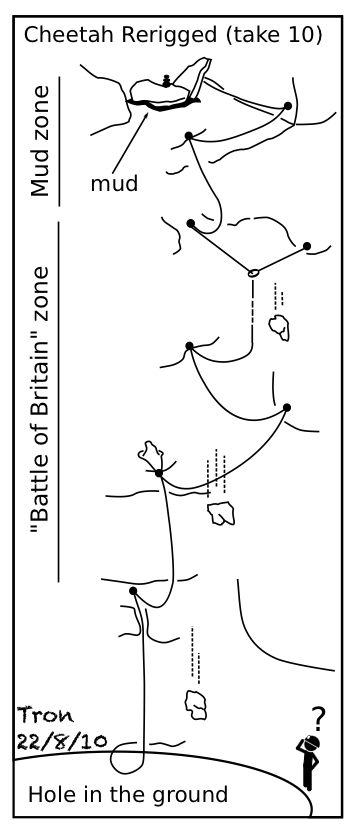
\includegraphics[width=\linewidth]{2010/ap_awards/Tharatorn Supasiti - March 2012 - rerigging-cheetah--orig.jpg}} 
 \caption{Rerigging \protect\passage{Cheetah}, again - and again - and again\ldots{} \pen{Tharatorn Supasiti}}
 \label{cheetah cartoon}
\end{marginfigure}


Kicked out of bed at seven by the night train, I gingerly put on cold caving gear, ate some fishy
cheesy soupy smash and headed off to '\passage{Wonderland}'. Unfortunately this involved an encounter with
the scariest pitch I have ever and hopefully will ever come across. Initially named \passage{Leopard} due to the
Leopard spot shaped mud splats on the walls, it soon became known instead as \passage{Cheatah}, due to that
fact that a successful passage elicits a feeling nothing less than one of cheating death. Whilst waiting
for the pitch to be rerigged in a safer fashion, a good deal of dancing was required to keep warm. The
caves after \passage{Cheatah} are majestic. Large amphitheatre-like holes, gloriously decorated passages and
chambers full of large rocks to climb over, wiggle between and slide under. The name \passage{Wonderland} was
well deserved.


However, as wondrous as it all was, exploring this only recently discovered cave and wandering
further and further away from camp really scared me. Sleeping so deep underground, waking up and
travelling even further into the abyss sent me a little crazy. Normal life has never seemed so far away.
Thankfully a new, never explored pitch was quickly rigged and as the newbie I was allowed to descend
first into the virgin cave. Fear was soon replaced with excitement, I would be the first person ever in
the history of everything to see and touch and just be in this part of the world. The pitch led to a
nice sized chamber with a stream way at the bottom. No waiting for the other two, I scampered into
the narrow passage, which became a pretty, winding stream way with crystal clear water and white
14
limestone. This ended with a pitch that ended our pushing (but began someone else's). After agreeing
on the name '\passage{Serpentine}', due to its snake-like meandering and association with the Serpentine Lake,
we began the arduous task of surveying the new cave. After surveying we headed back to camp, tired
and emotionally drained. \passage{Cheatah} was no more pleasant going up than coming down, the slippery
mud made it frustratingly tricky to reach the top. Glad to be back at camp.


After 6 hours of prussicking we made it for sunset and enjoyed the relaxed life of the plateau. The
next day the survey data was entered into the computer and we saw our new passage in 3D and linked
to the rest of the system. One week of caving and already 1.5km of cave had been discovered! Over the
next few days the rain came which kept the cavers underground and the rest of us huddled in the bivi.
\bignote{These days were dedicated to games of chess and cards}. After the rain had ceased I had a little trip
down \passage{system Migovec}, the more thoroughly explored system that it is hoped connects with \passage{Vrtnarija}.
We had a day dedicated to scaling the nearby peaks, which provided some exhilarating climbing. We
then travelled down to Tolmin and enjoyed luxuries such as pizza and swims in the emerald green
water of the \passage[river]{Soča} river.


\begin{figure*}
\checkoddpage \ifoddpage \forcerectofloat \else \forceversofloat \fi
\centering
    \begin{subfigure}{0.49\textwidth}
        \centering
        \frame{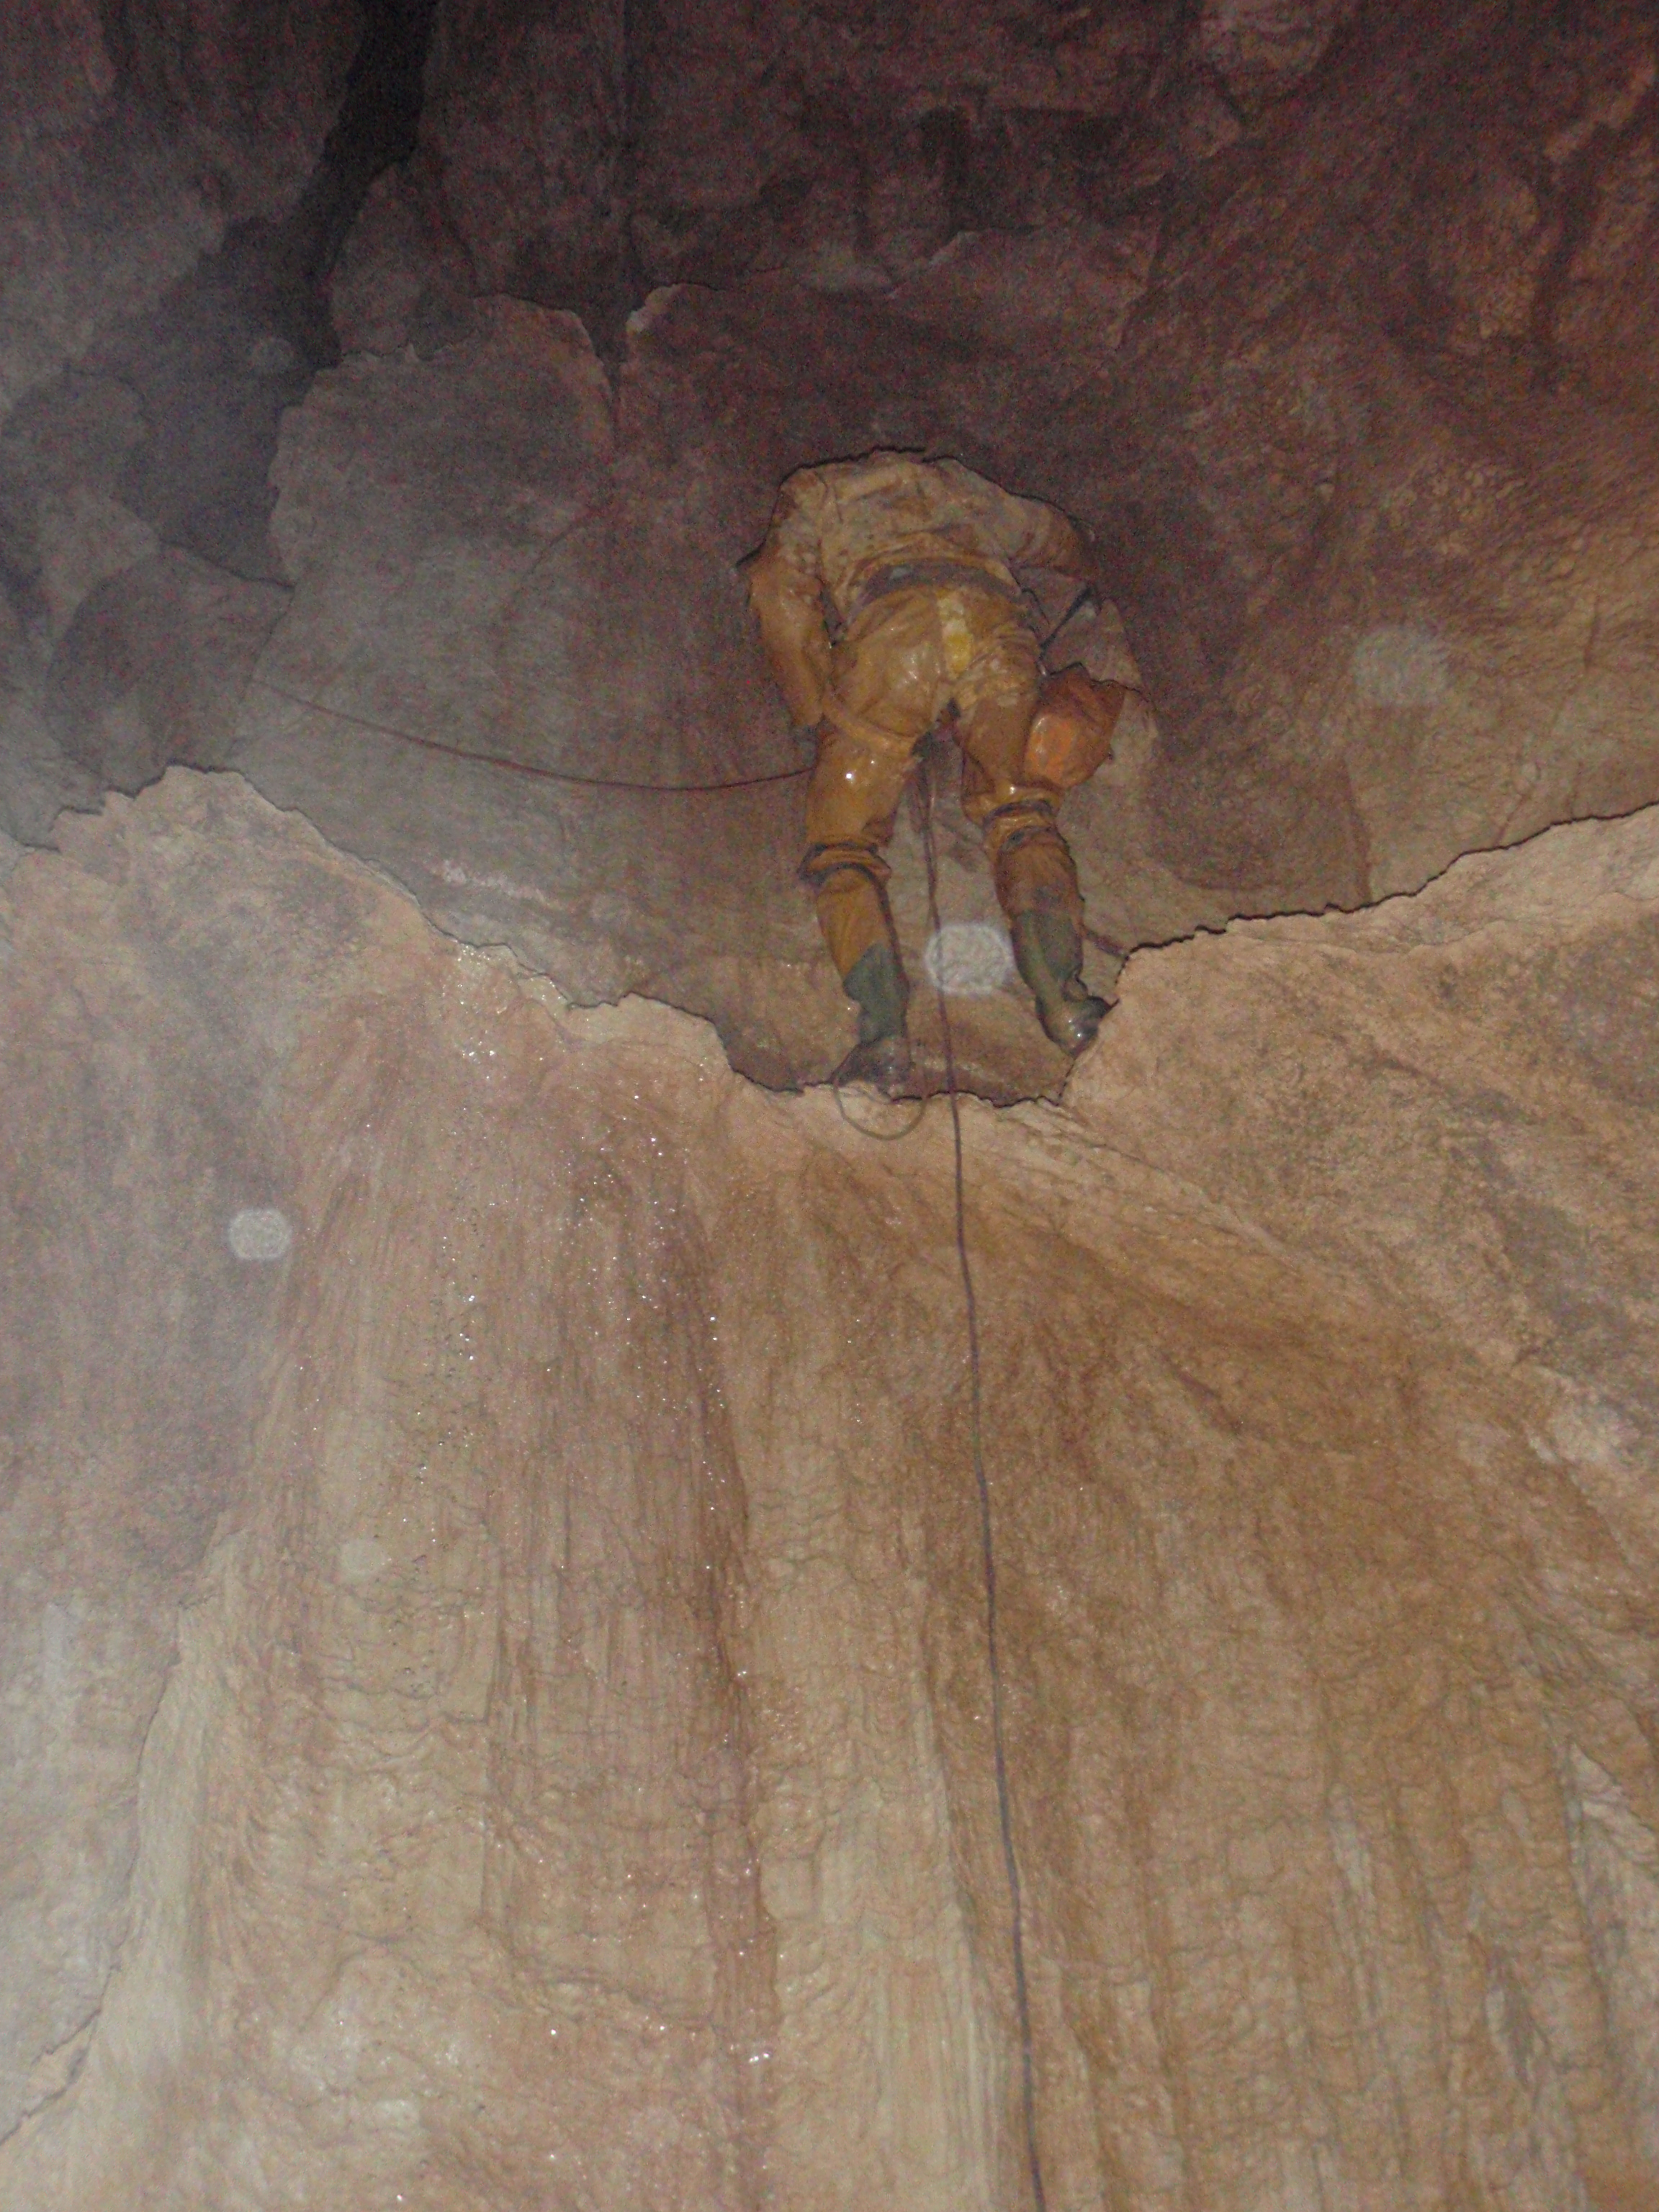
\includegraphics[width=\linewidth]{2010/ap_awards/20100728-21-43-22 - Iztok Mozir - P7284655 - Serpentine Pitch in the Albert Hall--orig.jpg}} 
        \caption{} \label{serpentine pitch}
    \end{subfigure}
        \hfill
\begin{subfigure}{0.49\textwidth}
\centering
\frame{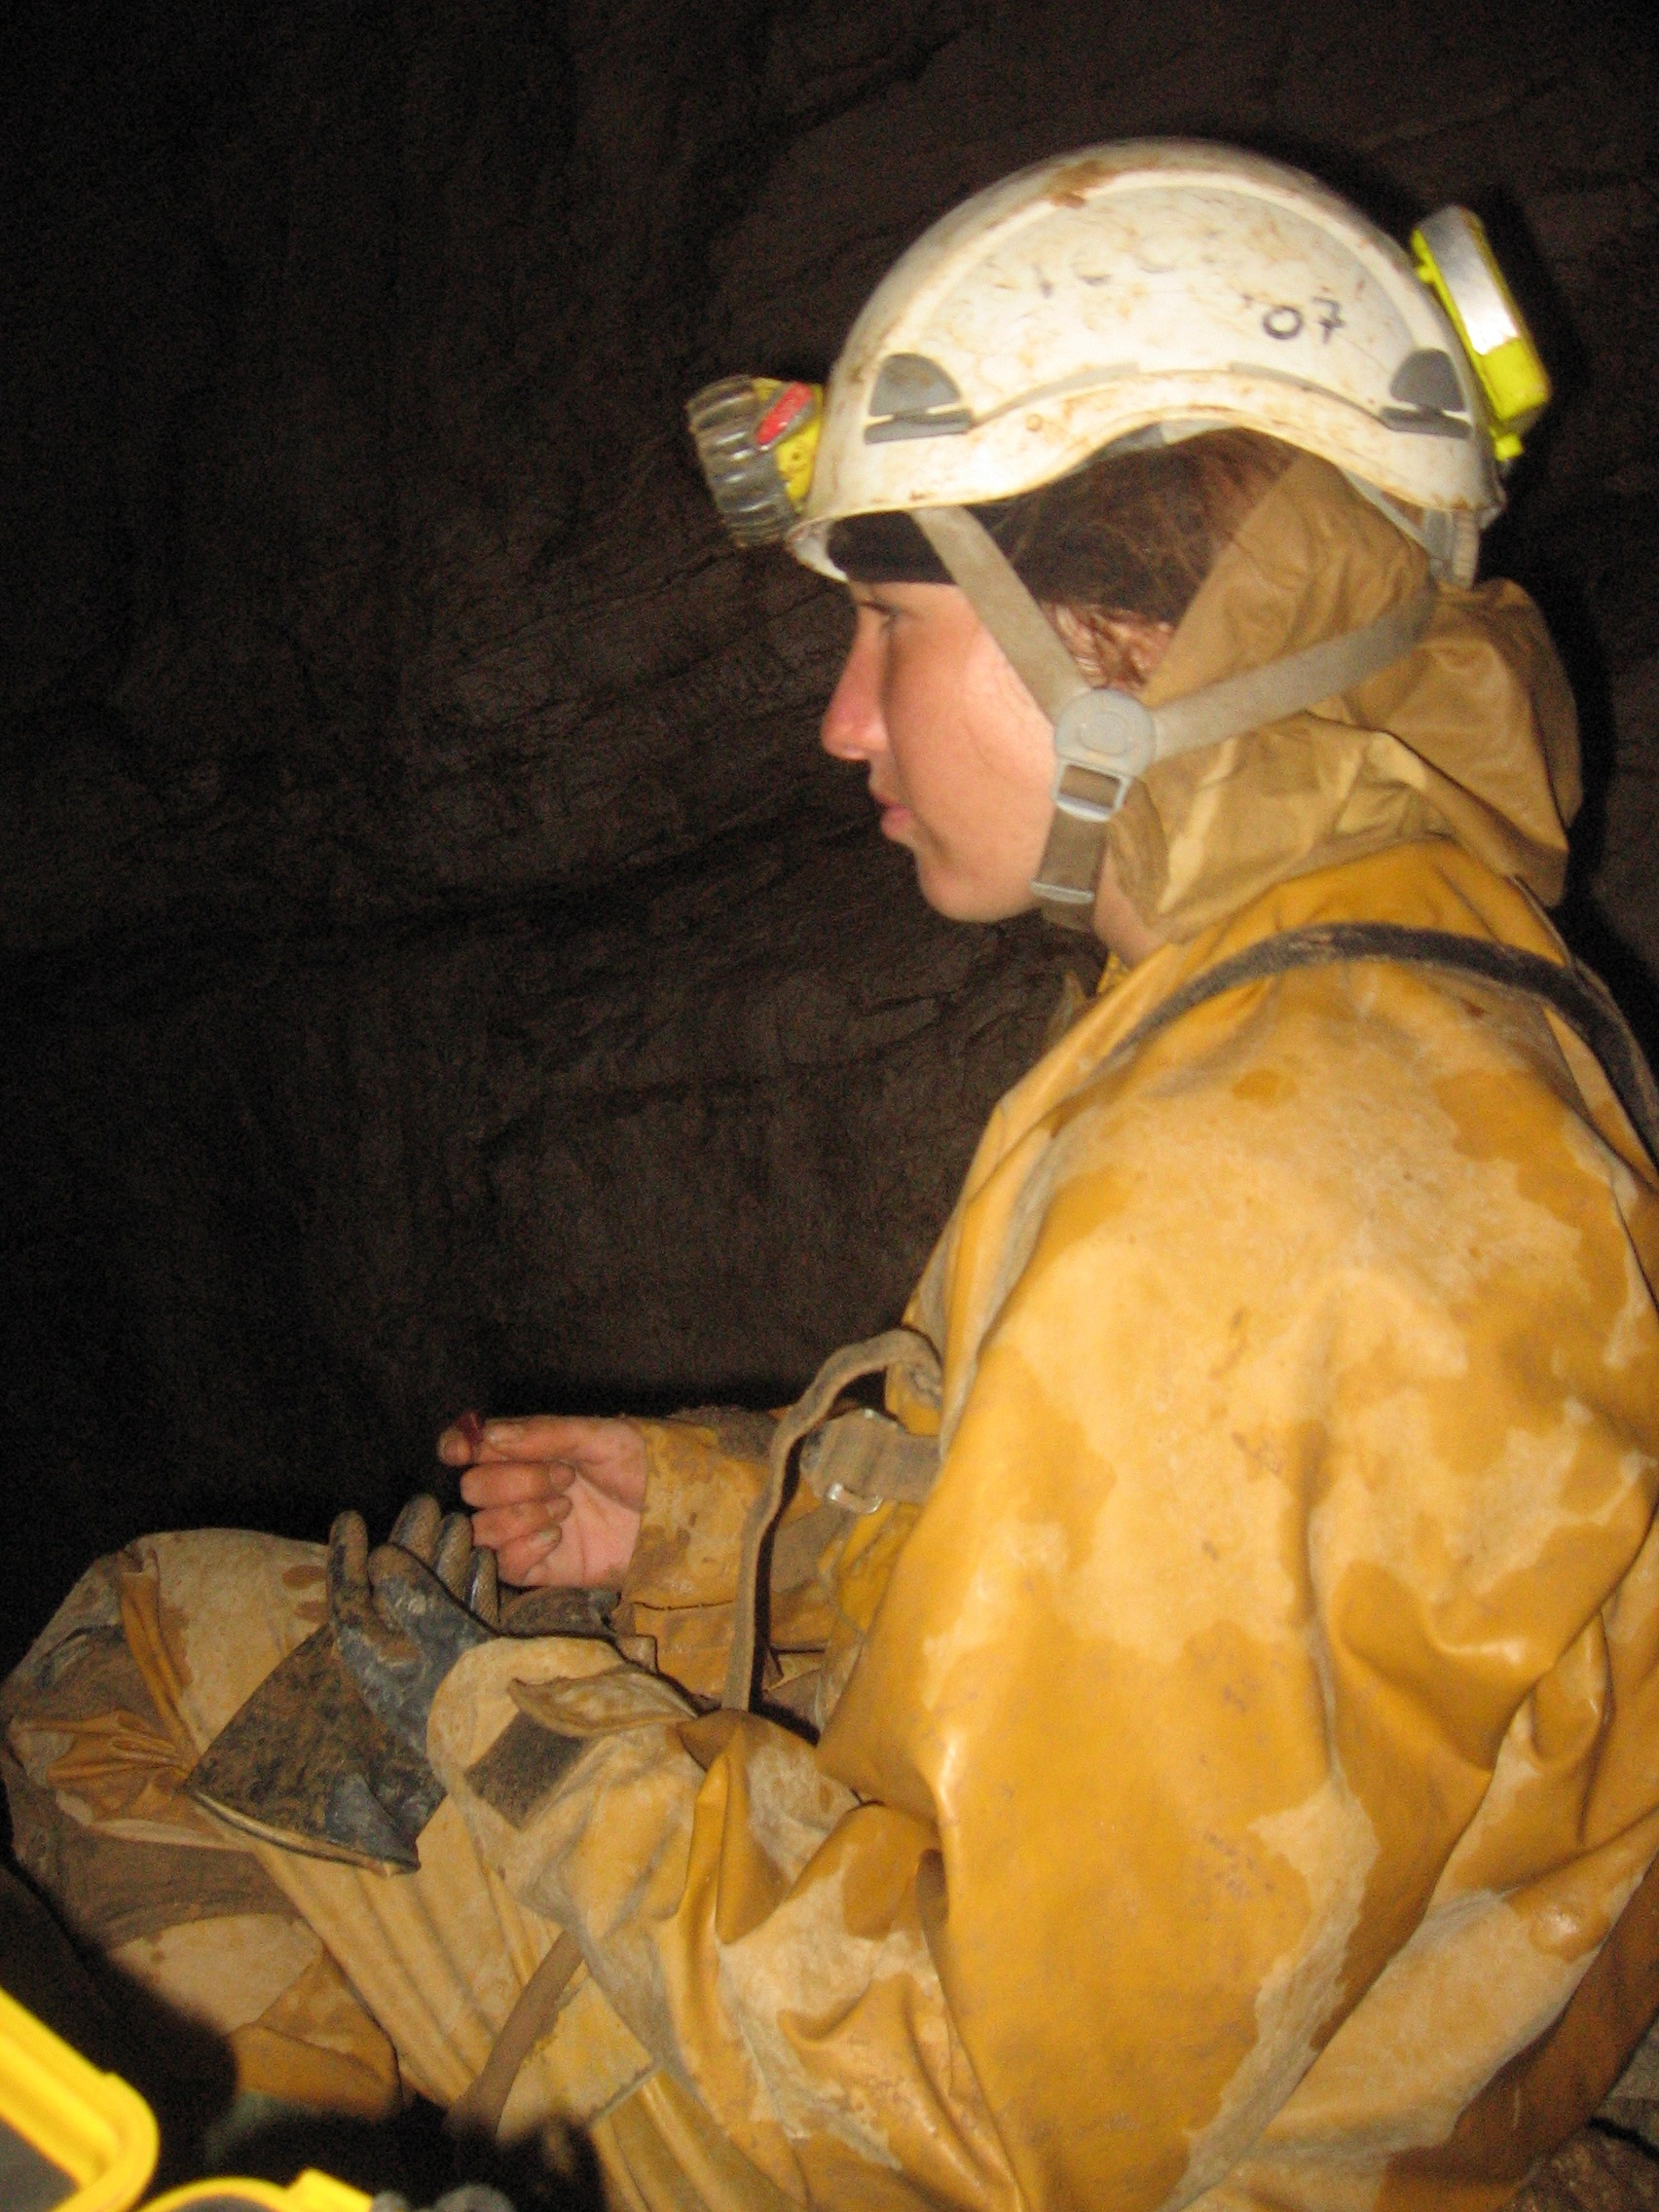
\includegraphics[width=\linewidth]{2010/ap_awards/20100809-15-47-45 - Jarvist Frost A520 - IMG_0017 - hanging out at bottom of zimmer--orig.jpg}}
 \caption{}\label{kate zimmer}
\end{subfigure}
  \caption{\textit{a}) Dan Greenwald on the \protect\passage{Serpentine} pitch. \pic {Iztok Mozir} \textit{b}) Kate at the bottom of \protect\passage{Zimmer}. \pic{Jarvist Frost}}
\end{figure*}


Showered and rejuvenated we headed back to the plateau, anxious to get back underground. Due
to the amount of interest from Slovenians and ICCC members alike to get in on the action it wasn't
till the final days of the caving period that I got to return to camp. Two of us were to pack up camp
and hopefully get some pushing done in-between. Camp was not as friendly as in the early days with
piles of litter, waiting to be carried out, tarnishing the once pure environment. After a long sleep with
no one on the night train to wake us up we reluctantly got out into the cold and made our way to
the pushing front. 
\margininbox{9/8/10 21:40}{
Back in camp, hurrah! Last night this year,
it's been good. Can't wait to come back next year if you all will have me.
\name{Kate Smith}}{\logbook}
Although we found no further leads I was given a tour of the majority of the new
findings this year. We saw some of the strangest formations such as several spirals of mud that looked
like a plug had been pulled beneath them. The huge rifts and chambers are glorious and lots of fun
to explore. We headed back to camp to finish the pack up and slept at camp for the final time this
year. Had my last serving of fishy soupy cheesy smash (Thank god!) and went on my way. Heading
out we met the various teams sent down to carry the remaining bags who made their presence known
with singing heard from many pitches away.



\begin{pagefigure}
\checkoddpage \ifoddpage \forcerectofloat \else \forceversofloat \fi
   \centering
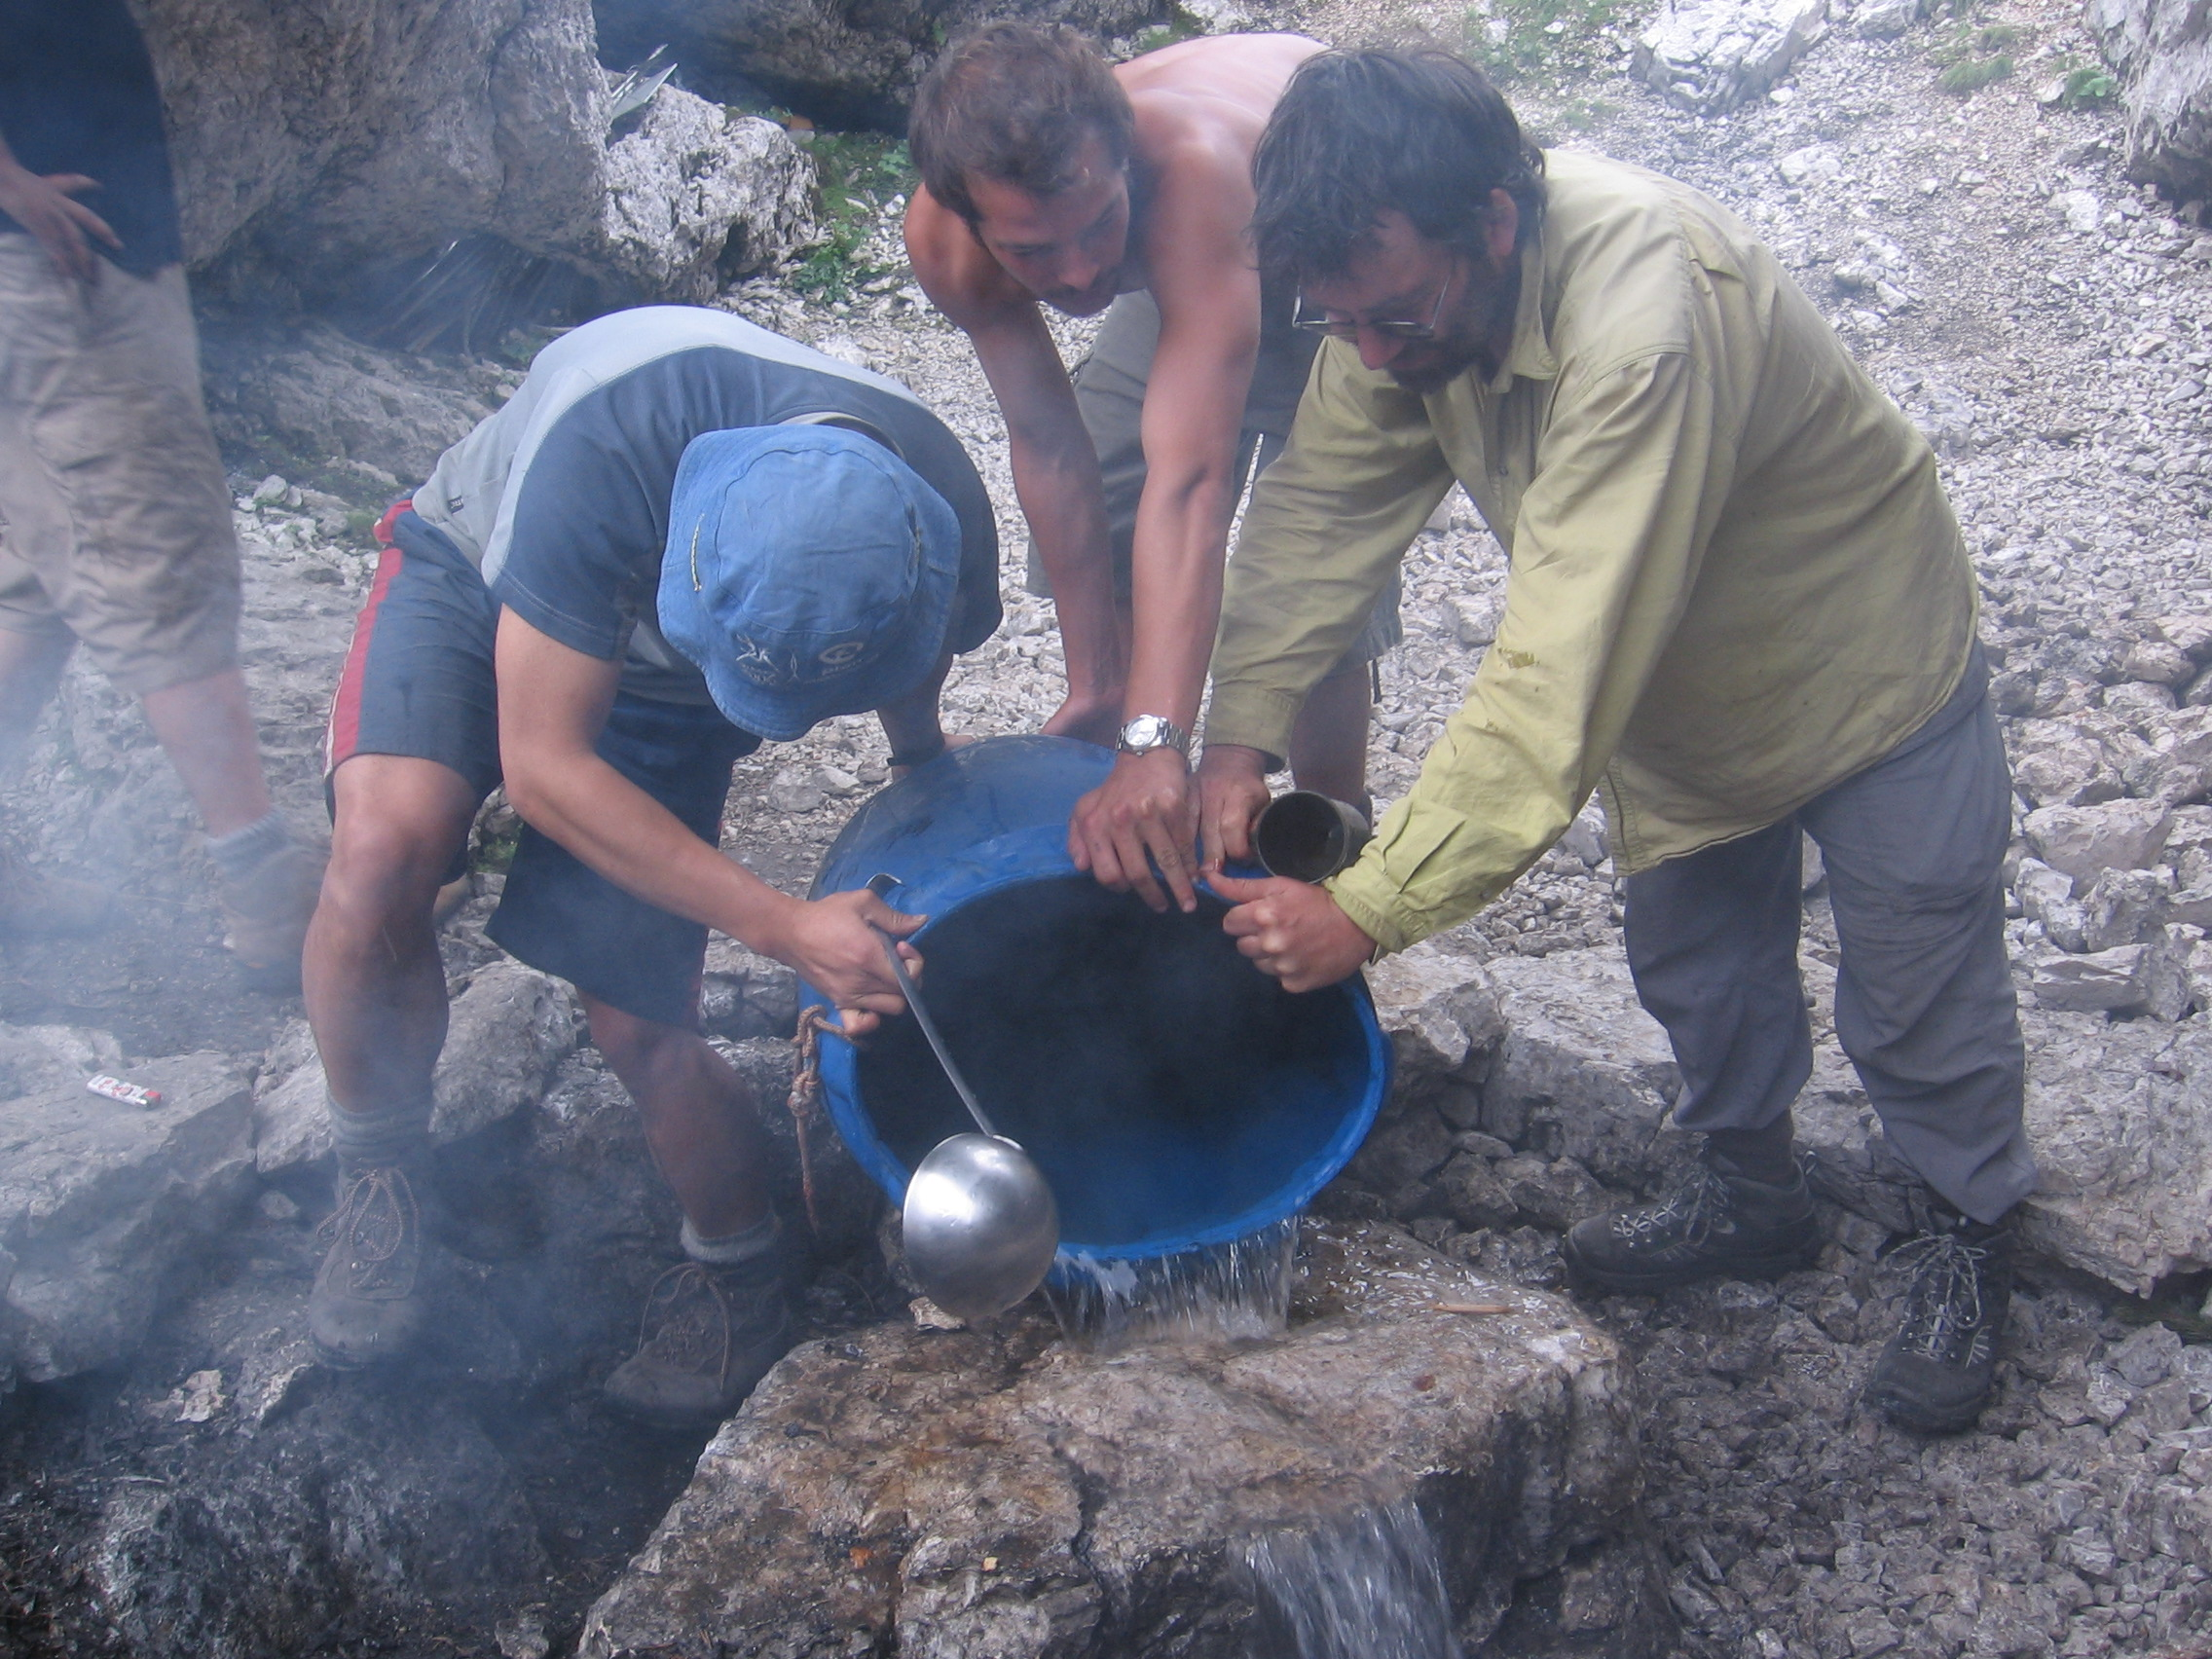
\includegraphics[width = \textwidth]{2010/ap_awards/20100812-13-11-19 - Jarvist Frost A520 - IMG_0046--orig.jpg}
\caption{Thara Supasiti, Myles Denton and Dave Wilson pouring the last of the collected rainwater over the stone table to wash it. \pic{Jarvist Frost}} \label{stone table wash}
\end{pagefigure}


\bignote{The next few days were spent packing away the bivi, removing all evidence of our presence} in the
national park. After saying goodbye to the plateau we travelled to \passage[town]Tolmin and stayed in a member's
flat. The next few days were spent giving presentations to the enthusiastic locals about our exploration. A total of 2.2km of new cave all below -550m left spirits on a high. A connection between the two
systems now looks ever more likely which, if found, would bring it close to being the longest cave in
Slovenia. On our final night we celebrated our achievements with the JSPDT with traditional Slovenian
music, dancing and drinking.

\tweet{7:12PM Aug 11th, 2010}{Cave\&UG camp fully derigged last night.Beaut weather for carries down,raspberries ripe. Stunning last sunset as an end to an epic expo. ICCC}


Very hungover, we packed the minibus and reluctantly left \passage[town]{Tolmin}. This will be an experience I
will never forget. Not only has my caving vastly improved and my thirst for caving increased but it
was the first of many caving expeditions I will be part of. The excitement of caving in new countries
will always enthuse me but I have the feeling that as many times as I may explore the deep caves of
\passage[mountain]{Tolminski Migovec} we will always have unfinished business.


\name{Kate Smith}